\documentclass[12pt,a4paper]{article}
\usepackage[OT4]{polski}
\usepackage[top=2.5cm, bottom=2.5cm, left=2cm, right=2cm]{geometry}
\usepackage{graphicx}
\usepackage{float}
\usepackage[colorlinks=true, linkcolor=blue]{hyperref}

\begin{document}

\title{Projekt na bazy danych 2023 - Dokumentacja}
\author{Paweł Packiewicz \and Adam Sochoń \and Dominik Ochej \and Bartosz Sabat \and Adrian Tomczak}
\maketitle
\tableofcontents
%%%%%%%%%%%%%%%%%%%%%%%%%%%%%%%%%%%%%%%%%%%%%%%%%%%%%
\section{Spis użytych technologii}
Podczas tworzenia projektu wykorzystane zostały różne narzędzia.
\subsection{Python}
Oraz biblioteki:
\begin{itemize}
\item \textbf{datetime},
\item \textbf{pandas} - wykorzystane podczas generowania dat,
\item \textbf{mysql} - wykorzystana do łączenia się z bazą,
\item \textbf{cvs} - wykorzystane do otwierania plików tekstowych,
\item \textbf{math},
\item \textbf{numpy},
\item \textbf{random} - wykorzystane podczas generowania różnych danych,
\item \textbf{itertools} - wykorzystane podczas analizy,
\item \textbf{matplotlib} - wykorzystane podczas generowania wykresów,
\item \textbf{os} - wykorzystane do nawigowania między plikami.
\end{itemize}

\subsection{MariaDb}
Jako dialekt MySql użyty do komunikacji z bazą danych.

\subsection{Git}
Jako narzędzie do kontroli wersji i pracy w grupie.

\section{Lista plików i opis zawartości}
Projekt zawiera 3 skrypty w folderze głównym:
\begin{itemize}
\item \textit{bob\_the\_builder.py}, który odpowiada za tworzenie, lub resetowanie bazy danych. Podczas tworzenia bazy uruchamia funkcje znajdujące się w pliku \textit{fill.py}.
\item \textit{drop\_all}, którym można usunąć wszystkie tabele z bazy danych.
\item \textit{Analiza\_danych.py}, który analizuję bazę danych.
\end{itemize}
Oprócz tego w folderze głównym znajdują się foldery:
\begin{itemize}
\item \textit{creators}, który zawiera moduły napisane w pythonie służące do tworzenia tabel w bazie.
\item \textit{generators}, który zawiera generatory losowych danych służące do uzupełniania danych w tabelach.
\item \textit{dokumentacja}, który zawiera tą dokumentację oraz pliki poboczne służące do jej generowania.
\end{itemize}
\section{Instrukcja uruchamiania}
By stowrzyć nową bazę i wypełnić ją danymi należy uruchomić plik \textit{bob\_the\_builder}(cały proces zajmuje niestety trochę czasu). By na podstawie danych znajdujących się obecnie w bazie wygenerować analizę należy uruchomić plik \textit{Analiza\_danych.py}. ...

\section{Schemat projektu bazy danych}
\begin{figure}[H]
\centering
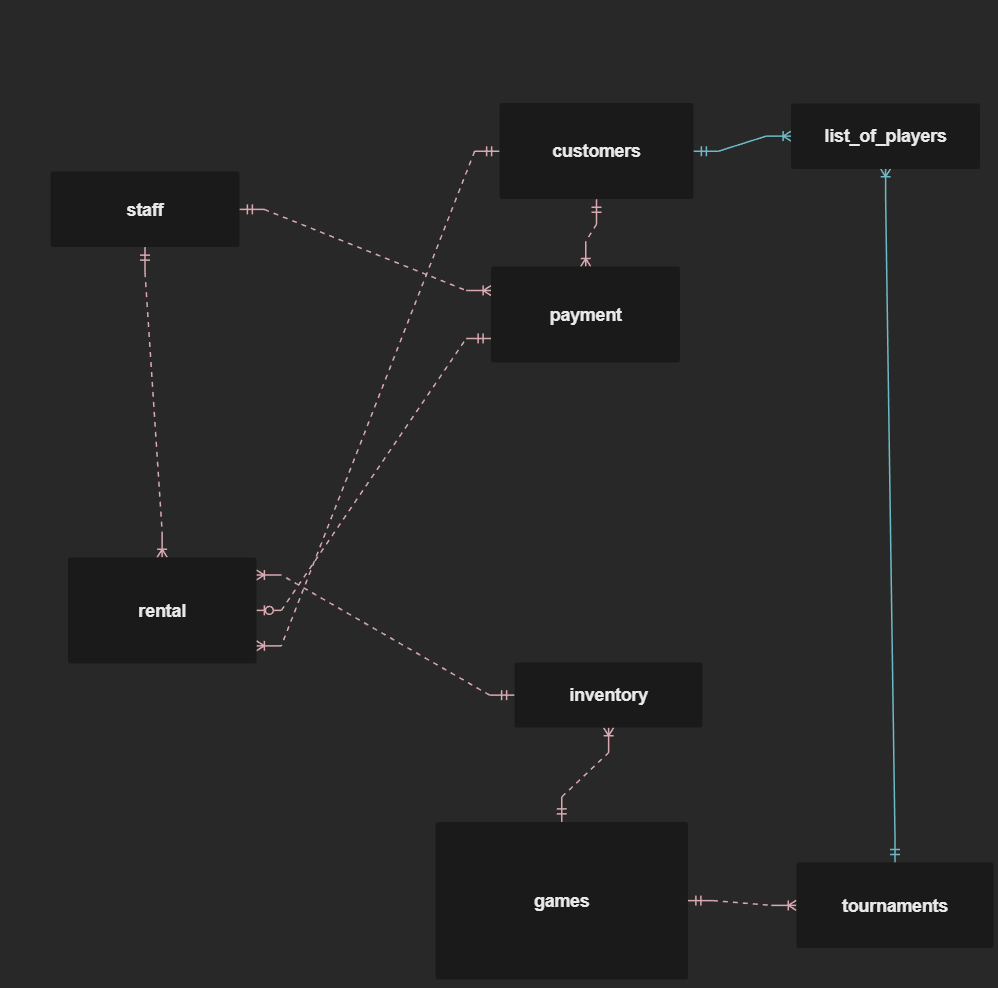
\includegraphics[width=150mm]{schemat.png}
\end{figure}

\section{Opis zależności funkcyjnych z wyjaśnieniem}
\subsection{Tabela \textit{customers}}
Kluczem głównym tabeli jest \textit{customer\_id}.

\subsection{Tabela \textit{games}}
Kluczem głownym jest \textit{game\_id}.
Na podstawie id każdej z gier generowana jest tabela \textit{inventory}.
Korzystając z informacji o liczbie graczy i czasie gry z każdej z gier generowana jest tabela dotycząca turniejów.

\subsection{Tabela \textit{inventory}}
Kluczem głównym jest \textit{inventory\_id}. \textit{game\_id} jest kluczem obcym odnoszącym się do \textit{game\_id} z tabeli \textit{games}.

\subsection{Tabela \textit{list\_of\_players}}
Tabela działa według założenia, że każdy gracz jest wpisywany do systemu jako klient by uprości zapis danych.
Tabela posiada dwa klucze główne będące jednocześnie kluczami obcymi \textit{customer\_id} oraz \textit{tournament\_id} łącząc tym samym informacje o zawodnikach i turniejach.

\subsection{Tabela \textit{staff}}
Kluczem głównym jest \textit{staff\_id}. Tabela nie posiada kluczy obcych.

\subsection{Tabela \textit{rental}}
\textit{rental\_id} jest kluczem głównym tabeli.
Tabela posiada 3 klucze obce \textit{inventory\_id}, \textit{customer\_id} oraz \textit{staff\_id} odnoszące się do kluczy głównych tabel \textit{inventory}, \textit{customer}, \textit{staff}.

\subsection{Tabela \textit{payment}}
\textit{payment\_id} jest kluczem głównym tabeli.
Tabela posiada klucze obce \textit{rental\_id}, \textit{customer\_id} i \textit{staff\_id}.

\subsection{Tabela \textit{tournaments}}
\textit{tournament\_id} jest kluczem głównym tabeli.
Tabela posiada klcz obcy \textit{game\_id}. Dane w tabeli są generowane na podstawie gry, na której opraty jest dany turniej.


\section{Uzasadnienie dotyczące EKNF}


\section{Trudności podczas tworzenia projektu}
Największą trudnością było dogadanie się jak powinien wyglądać schemat bazy. Trudno było się też zorientować jak
uzupełniać bazę za pomocą connectora do pythona. Dużo trudności sprawiło też sensowne stworzenie danych tak by tabele
odnoszące się do siebie miały sens.

\end{document}